% !TEX root = CSL 2021.tex

 

\begin{figure}
\begin{subfigure}{0.45\textwidth}
\parbox[h][4.6cm][c]{\textwidth}{
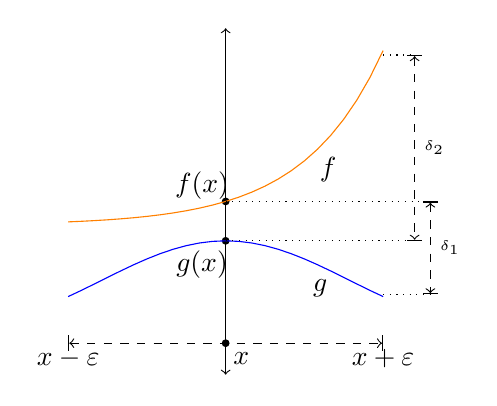
\begin{tikzpicture}[domain=-2:2]
%\draw[very thin,color=gray] (-0.1,-1.1) grid (3.9,3.9);
\draw[dashed, |<->|]   (-2,0) -- (2,0);
\draw[<->] (0,-0.4) -- (0,4); % node[above] {$f(x)$};

    \node at (0,0)[circle,fill,inner sep=1pt]{};
%    \node at (-2,0)[circle,fill,inner sep=1pt]{};
%    \node at (2,0)[circle,fill,inner sep=1pt]{};
\node(z) at (0.2,-0.2) {$x$};
\node(-e) at (-2,-0.2) {$x-\varepsilon$};
\node(e) at (2,-0.2) {$x+\varepsilon$};


\node(f) at (0,0.8+0.5)[circle,fill,inner sep=1pt]{};
\node(f) at (0,1.5+0.3)[circle,fill,inner sep=1pt]{};

\node(f) at (-0.3,2) {$f(x)$};

\node(f) at (-0.3,1) {$g(x)$};


\node(ff) at (1.3,2.2) {{$f$}};
\node(gg) at (1.2,0.7) {{$g$}};

%\draw[color=red] plot (\x,\x) node[right] {$f(x) =x$};
% \x r means to convert ?\x? from degrees to _r_adians:
\draw[color=blue] plot (\x,{0.8+ 0.5*(cos(\x r))}) ;
\draw[color=orange] plot (\x,{1.5+0.3*exp(\x)}) ;

\draw[dotted] (0,1.8) -- (2.6,1.8);
\draw[dotted] (2,0.62) -- (2.6,0.62);
\draw[dotted] (0,1.3) -- (2.4,1.3);
\draw[dotted] (2,3.66) -- (2.4,3.66);

%
%\draw[dotted] (0,1.8) -- (2, 0.62);
%\draw[dotted] (0,1.3) -- (2, 3.66);

\draw[dashed,|<->| ] (2.4,3.66) -- node[right] {\tiny$\delta_{2}$} (2.4,1.3);
\draw[dashed,|<->| ] (2.6,1.8) -- node[right] {\tiny$\delta_{1}$} (2.6,0.62);

\end{tikzpicture}
}
\caption{\small In differential logical relations the distance between two functions $f,g:\R\to \R$, computed in $(x,\varepsilon)$ is the maximum between 
$\delta_{1}=\max\{d(f(x),g(y));~ y\in [x-\varepsilon, x+\varepsilon]\}$ and 
$\delta_{2}=\max\{d(g(x), f(y));~ y\in [x-\varepsilon, x+\varepsilon]\}$.}
% and 
%
%
%minimum $\delta$ such that for all $y\in [x-\varepsilon, x+\varepsilon]$, both $g(y)\in [f(x)-\delta, f(x)+\delta]$ and $f(y)\in[g(x)-\delta, g(x)+\delta]$ hold. $\delta$ is thus $\max\{\delta_{1},\delta_{2}\}$ in the image above.}
\label{fig:graph1}
\end{subfigure} \ \ \ \ 
\begin{subfigure}{0.45\textwidth}
\parbox[h][4.6cm][c]{\textwidth}{
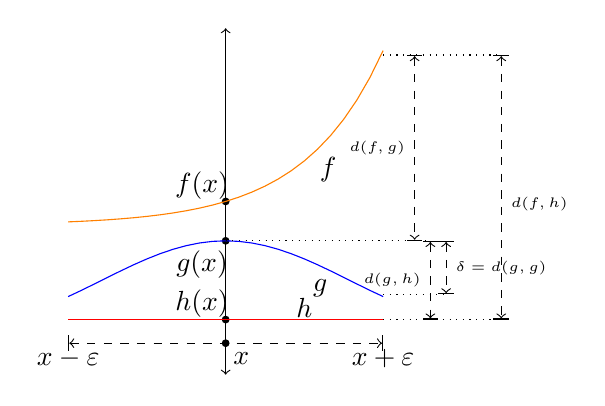
\begin{tikzpicture}[domain=-2:2]
%\draw[very thin,color=gray] (-0.1,-1.1) grid (3.9,3.9);
\draw[dashed, |<->|]   (-2,0) -- (2,0);
\draw[<->] (0,-0.4) -- (0,4); % node[above] {$f(x)$};

    \node at (0,0)[circle,fill,inner sep=1pt]{};
%    \node at (-2,0)[circle,fill,inner sep=1pt]{};
%    \node at (2,0)[circle,fill,inner sep=1pt]{};
\node(z) at (0.2,-0.2) {$x$};
\node(-e) at (-2,-0.2) {$x-\varepsilon$};
\node(e) at (2,-0.2) {$x+\varepsilon$};


\node(f) at (0,0.8+0.5)[circle,fill,inner sep=1pt]{};
\node(f) at (0,1.5+0.3)[circle,fill,inner sep=1pt]{};
\node(f) at (0,0.3)[circle,fill,inner sep=1pt]{};

\node(f) at (-0.3,2) {$f(x)$};

\node(f) at (-0.3,1) {$g(x)$};

\node(f) at (-0.3,0.5) {$h(x)$};

\node(ff) at (1.3,2.2) {{$f$}};
\node(gg) at (1.2,0.7) {{$g$}};
\node(gg) at (1,0.45) {{$h$}};

%\draw[color=red] plot (\x,\x) node[right] {$f(x) =x$};
% \x r means to convert ?\x? from degrees to _r_adians:
\draw[color=blue] plot (\x,{0.8+ 0.5*(cos(\x r))}) ;
\draw[color=orange] plot (\x,{1.5+0.3*exp(\x)}) ;
\draw[color=red] plot (\x,{0.3}) ;



\draw[dotted] (0,1.3) -- (2.6,1.3);
\draw[dotted] (2,0.3) -- (3.5,0.3);
\draw[dotted] (0,1.3) -- (2.4,1.3);
\draw[dotted] (2,3.66) -- (3.5,3.66);
\draw[dotted] (2,0.62) -- (2.8,0.62);

%
%\draw[dotted] (0,1.8) -- (2, 0.62);
%\draw[dotted] (0,1.3) -- (2, 3.66);

\draw[dashed,|<->| ] (2.4,3.66) -- node[left] {\tiny$d(f,g)$} (2.4,1.3);
\draw[dashed,|<->| ] (2.6,1.3) -- node[left] {\tiny$d(g,h)$} (2.6,0.3);

\draw[dashed,|<->| ] (2.8,1.3) -- node[right] {\tiny$\delta=d(g,g)$} (2.8,0.62);

%\draw[dashed,|<->| ] (3.5,2.96) -- node[above right] {\tiny$\begin{matrix}d(f,g)+d(g,h)\\ -d(g,g)\end{matrix}$} (3.5,0.3);

\draw[dashed,|<->| ] (3.5,3.66) -- node[below right] {\tiny$d(f,h)$} (3.5,0.3);

\end{tikzpicture}
}
%
\caption{\small The metric of differential logical relations is not a partial metric: the example above shows that $d(f,h)> d(f,g)+d(g,h)- d(g,g)$ (with all distances computed in $(x,\varepsilon)$). \\ \ }% and 
%
%
%minimum $\delta$ such that for all $y\in [x-\varepsilon, x+\varepsilon]$, both $g(y)\in [f(x)-\delta, f(x)+\delta]$ and $f(y)\in[g(x)-\delta, g(x)+\delta]$ hold. $\delta$ is thus $\max\{\delta_{1},\delta_{2}\}$ in the image above.}
\label{fig:graph2}
\end{subfigure}
\end{figure}


The first compositional formalization of approximate program transformations we are aware of is the one in \cite{chaudhuri}, where an explicit distinction is made between exact and approximate programs by 
associating, with each type $A$ of System F, a suitable type of approximated programs. While no
explicit mention of a  metric structure is made in that paper, it is not difficult to see that most examples presented in \cite{chaudhuri} can be suitably reformulated in our framework. 
%Moreover, the emphasis on typing rules for program distances 
%suggests to look for a similar   for our semantical language of approximate functions.

A more semantic framework is presented in recent work by Dal Lago, Gavazzo and Yoshimizu on \emph{differential logical relations} \cite{dallago:differential-stlc}. While following some ideas from \cite{chaudhuri}, \cite{dallago:differential-stlc} 
emphasize the need to define a metric space over simple types. To this end introduces, the idea of varying the quantales in which distances are measured is introduced as  a key ingredient to obtain a cartesian closed category. In such category all objects are endowed with the structure of a \emph{generalized metric domain}, obtained by a suitable weakening of usual metric axioms.

However, there seems to be no way of obtaining a standard metric structure based on differential logical relations. We can show this fact with a simple example. In such model the distance between two programs 
 $f,g:\mathsf{Real}\to \mathsf{Real}$ is taken in the quantale of functions from $\R\times \R_{+}^{\infty}$ to $\R_{+}^{\infty}$: intuitively, 
  $d(f,g)$ associates a closed interval $[x-\epsilon,x+\epsilon]$ (corresponding to the pair $(x,\varepsilon)$) with the smallest distance $\delta$ such that $[ f(x)-\delta, f(x)+\delta]$ and $[g(x)-\delta,g(x)+\delta]$ both contain the images of $[x-\varepsilon, x+\varepsilon]$ through
 $g$ and $f$ respectively (see Fig. \ref{fig:graph1}). 
%  The fact that $\diff (f)$ associates an interval $I=[x-\varepsilon, x+\varepsilon]$ with the smallest interval \emph{centered in $f(x)$} containing the image of $I$ forces an unwanted loss of precision. This can already be seen in Fig. \ref{fig:graph2}: 
%
As shown in Fig. \ref{fig:graph2}, by letting $\delta=d(g,g)(x,\varepsilon)$, we have that $d(g,g)$ sends the interval $I=[x-\varepsilon, x+\varepsilon]$ onto the interval $[g(x)-\delta, g(x)+\delta]$, which has diameter $2\delta$, while the image of $I$ has diameter $\delta$, making the triangular law of partial metrics fail. 



